\section[Описание деталей реализации]{ОПИСАНИЕ ДЕТАЛЕЙ РЕАЛИЗАЦИИ}

\subsection{Установка программного обеспечения}
\label{sub:realization_software_install}

Для разработки интернет-магазина с учётом выбранных разделе~\ref{sec:choice}
технологий установим следующие программы:

\begin{itemize}
  \item MySQL 5.5;
  \item Apache Tomcat 7;
  \item Apache Maven 3;
  \item Git.
\end{itemize}

На рисунке~\ref{lst:software_install} представлены команды установки данных
программ в ОС семейтса Linux.

\begin{lstlisting}[caption=Команды установки необходимого программного обеспечения,label=lst:software_install]
sudo apt-get install mysql-client mysql-server
sudo apt-get install tomcat7
sudo apt-get install maven
sudo apt-get install git
\end{lstlisting}


\subsection{Создание проекта и настройка компонентов}

Создадим базу данных, которую будем использовать для хранения сущностей интернет-магазина.
Код создания базы данных, используемой в разрабатываемом проекте,
продемонстрирован на рисунке~\ref{lst:db_create}.

\begin{lstlisting}[caption=Команды создания базы данных для проекта,label=lst:db_create]
mysql -u root -p
<password>
create database bikeshopdb default character set utf8;
exit;
\end{lstlisting}

Таблицы создавать не нужно, при сборке проект сам будет проверять есть ли
необходимые таблицы. Если их нет, они будут созданы.

Далее создадим в Intellij IDEA проект, поддерживающий технологию Java EE.
В настройках проекта укажем путь к установленному Apache Maven,
настроим использование системы контроля версий git.

В корне проекта создадим папку \textit{src}, в ней будет храниться весь исходный
код разрабатываемого приложения; В папке src создадим папку \textit{main}, в ней ---
папки \textit{java}, \textit{resources} и \textit{webapp}.

Папка \textit{java} будет содержать весь исходный код приложения, написанный на Java.

В папке \textit{resources} разместим необходимые файлы с настройками приложения.

Папка \textit{webapp} будет содержать web-страницы, файлы описания стилей, и другие файлы,
относящиеся к клиентской части приложения.

В корне проекта создадим файл \textit{pox.xml}, он будет использоваться для
конфигурирования зависимостей Apache Maven. Содержимое данного файла
приведено в приложении~А.

В папке resources создадим файл \textit{app.properties}. В нём опишем настройки
соединения с базой данных, а также основные настройки библиотеки Hibernate.
Содержимое файла app.properties представлено на рисунке~\ref{lst:app_properties}.

\begin{lstlisting}[caption=Содержимое файла app.properties,label=lst:app_properties]
#DB properties
db.driver=com.mysql.jdbc.Driver
db.url=jdbc:mysql://localhost:3306/bikeshopdb
db.username=<username>
db.password=<password>

#Hibernate configuration
hibernate.dialect=org.hibernate.dialect.MySQLDialect
hibernate.show_sql=true
entitymanager.packages.to.scan=com.anash.bikeshop.entity
hibernate.hbm2ddl.auto=createentitymanager.packages.to.scan=com.anash.bikeshop.entity
\end{lstlisting}

\newpage

\subsection{Разработка серверной части приложения}

Приступим к описанию сущностей приложения. В папке \textit{java} создадим пакет
\textit{com.anash.bikeshop}, в нём --- пакет \textit{entity}. В данном пакете опишем
все сущности разрабатываемого интернет-магазина. Создадим классы
\textit{Bicycles, AvailableBicycles, Orders, OrdersArchive} и \textit{Users}.

Для того, чтобы связать описываемые сущности с базой данных будем использовать
\textit{аннотации}. Аннотации в Java --- специальная форма синтетических метаданных,
которая добавляется в исходный код приложения. Аннотации дают необходимую информацию
для компилятора, библиотеки Hibernate и прочих инструментов разработки~\cite{jpa_entities_design}.

В разрабатываемом проекте будут использованы аннотации, предоставляемые библиотекой
Hibernate, фреймворком Spring, а также встроенные в язык java (javax.persistence).
Пример использования аннотации для сущности Users разрабатываемого интернет-магазина
проиллюстрирован на рисунке~\ref{lst:users_entity}. Полный исходный код описания
сущности Users представлен в приложении~Б.

\begin{lstlisting}[caption=Пример использования Java-аннотаций,label=lst:users_entity]
@Entity
@Table(name = "users")
public class Users implements Serializable {
    @Id
    @GeneratedValue(generator = "increment")
    @GenericGenerator(name = "increment", strategy = "increment")
    @Column(name = "id", length = 6, nullable = false)
    private long id;

    @Email
    @NotNull
    @Column(name = "email", nullable = false)
    private String email;

    ...
}
\end{lstlisting}

После описания всех сущностей можно приступать к определению классов и интерфейсов,
отвечающих за доступ к данным. Создадим пакеты \textit{service} и \textit{repository}.

Пакет \textit{repository} содержит интерфейсы, которые предоставляет Spring Framework.
Они отвечают за непосредственную работу с данными. Содержимое файла UsersRepo.java
представлено на рисунке~\ref{lst:users_repo}.

\begin{lstlisting}[caption=Содержимое файла UsersRepo.java,label=lst:users_repo]
package com.anash.bikeshop.repository;

import com.anash.bikeshop.entity.Users;
import org.springframework.data.jpa.repository.JpaRepository;

public interface UsersRepo
        extends JpaRepository<Users, Long> {
}
\end{lstlisting}

Пакет \textit{service} содержит интерфейсы и их реализацию, предоставляющие доступ
к данным посредством использования соответствующих репозиториев.

Создадим интерфейс
\textit{Service} и объявим в нём методы, представленные на рисунке~\ref{lst:service}.

\begin{lstlisting}[caption=Объявленные в интерфейсе Service методы,label=lst:service]
void create(Type entity);
void update(Type entity);
void delete(Type entity);
Type getById(long id);

List<Type> getAll();
\end{lstlisting}

Затем создадим интерфейсы \textit{BicyclesService, AvailableBicyclesService,
OrdersService, OrdersArchiveService} и \textit{UsersService}, и унаследуем их от
интерфейса Service.

Полный исходный код реализации интерфейса \textit{UsersService} приведен в приложении~В.

После описания сервисов и репозиториев для доступа к данным можно приступать
к написанию контроллеров. В контроллерах будем описывать методы, которые будут
вызываться в зависимости от перехода на конкретные страницы. Создадим пакет
\textit{controller}, в котором будем сохранять необходимые контроллеры. Пример описания
контроллера представлен на рисунке~\ref{lst:controller}.

\begin{lstlisting}[caption=Пример описания контроллера BicycleController,label=lst:controller]
@Controller
public class BicycleController {

    @Autowired
    private BicycleService bicycleService;

    @RequestMapping(value = "/catalog/detail/{id}",
                    method = RequestMethod.GET)
    public ModelAndView bicycleDetail(@PathVariable Long id)
    {
        ModelAndView mav = new ModelAndView("detail");

        Bicycles bicycle = bicycleService.getById(id);
        mav.addObject("bicycle", bicycle);

        return mav;
    }

    ...
}
\end{lstlisting}

Из рисунка~\ref{lst:controller} видно, что мы используем BicycleService в качестве ресурса
для данного контроллера. При переходе
со страницы \textit{/catalog} на страницу с детальным просмотром конкретного велосипеда
\textit{/calalog/detail/\{id\}} будет вызван метод \textit{bicycleDetail()}, который принимает в
качетсве параметра \textit{id} велосипеда. В четырнадцатой строке происходит передача параметра
на страницу jsp с именем \textit{"bicycle"}.

Также стоит отметить наличие пакета \textit{config} в пакете \textit{com.anash.bikeshop}.
В нём располагаются основные конфигурации библиотеки Hibernate и отображения web-страниц.

Таким образом мы получаем структуру проекта, аналогичную представленной
на рисунке~\ref{fig:project_structure}.

\begin{figure}[h]
  \centering
  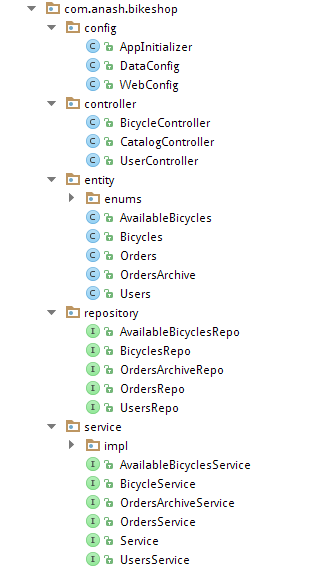
\includegraphics[width=80mm]{pic/project_structure.png}
  \caption{Структура пакетов \\ серверной части приложения}
  \label{fig:project_structure}
\end{figure}

\subsection{Разработка клиентской части приложения}

Создадим структуру папок для клиентской части приложения. В папке \textit{webapp}
создадим две папки: \textit{WEB-INF} и \textit{resources}.

Директория \textit{resources} будет содержать ресурсы веб-страниц,
такие как, например, файлы стилей и фотографии велосипедов.

В директории \textit{WEB-INF} создадим папки \textit{templates} и \textit{content}.
Папка \textit{templates} будет содержать общие элементы для всех страниц сайта,
такие как header, footer и др.

Перед созданием JSP-страниц разработаем макеты всех страниц для разрабатываемого
интернет-магазина. Макет страницы \textit{login.jsp} приведен
на рисунке~\ref{fig:wireframe_login}.

\begin{figure}[h]
  \centering
  
\includegraphics[width=160mm]{pic/login_template.png}
  \caption{Макет страницы \textit{login.jsp}}
  \label{fig:wireframe_login}
\end{figure}

После создания макетов всех JSP страниц можно приступать к вёрстке этих страниц.
Для вёрстки будем использовать следующий стек технологий: HTML, CSS, JSTL.

Для передачи параметров JSP странице могут использоваться \textit{скриплеты}
или \textit{JSTL}.

\textit{Скриплеты} --- часть кода программы, написанного только на одном языке.
JSP-скриплеты вставляются в код JSP-страницы в следующем виде:
\textit{<\% Java-код \%>}.

\textit{JSTL} --- стандартная библиотека тегов JSP. Теги JSP используются
для общих нужд, таких как разбор XML данных, условная обработка, создание циклов и
поддержка интернационализации.

\pagebreak

Пример использования языка JSTL на странице \textit{<<catalog.jsp>>}
представлен на рисунке~\ref{lst:jstl_example}.

\begin{lstlisting}[caption=Пример использования JSTL на странице \textit{catalog.jsp}, label=lst:jstl_example]
<%@ taglib prefix="c" uri="http://java.sun.com/jsp/jstl/core" %>

<div class="list">
  <c:forEach var="bicycle" items="${bicycles}" >
    <div class="list-row">
      <div class="list-title">
        <h2>${bicycle.manufacturer} ${bicycle.productName} (${bicycle.year})</h2>
      </div>
      ...
    </div>
  </c:forEach>
</div>
\end{lstlisting}

Результат отображения страницы \textit{login.jsp} представлен на рисунке~\ref{fig:login_jsp}

\begin{figure}[h]
  \centering
  
\includegraphics[width=160mm]{pic/login_site.png}
  \caption{Результат отображения страницы \textit{login.jsp} \\ в браузере}
  \label{fig:login_jsp}
\end{figure}

Легко убедится в том, что желаемый результат получен --- итоговая страница \textit{login.jsp}
полностью совпадает с разработанным ранее макетом.

Аналогичным образом были спроектированы все остальные страницы интернет-магазина.

\pagebreak
